\documentclass[12pt,a4paper]{report}
\usepackage{graphicx}
\usepackage{amsmath}
\usepackage{fancyhdr}
\usepackage{cite}
\usepackage{framed}
\usepackage{a4wide}
\usepackage{float}
\usepackage{blindtext}
\usepackage{multicol}
\usepackage{tabto}
\usepackage{amssymb}
\usepackage{doi}
\usepackage{biblatex}
%\usepackage{natbib}
%The below Section make chapter and its name to center of the page
\usepackage{blindtext}
\usepackage{xpatch}
\usepackage{mathptmx}
\usepackage{geometry}
\usepackage{xcolor}
\usepackage{tcolorbox}
\usepackage{bbold}
\usepackage{mathtools}
\usepackage{hyperref}
 \geometry{
 right=25mm,
 left=35mm,
 top=25mm,
 bottom=25mm,
 }
% \usepackage{fontspec}
\usepackage{tocloft}
\makeatletter
\renewcommand{\cftdot}{}
\renewcommand{\cftchappresnum}{CHAPTER }
\renewcommand{\cftchapaftersnum}{:}
\renewcommand{\cftchapnumwidth}{6.5em}
\renewcommand\cftfigindent{0pt}
\renewcommand\cftfigpresnum{Figure\ }
\renewcommand\cftfigaftersnum{ : }
\renewcommand{\cftfignumwidth}{5.5em}
\renewcommand{\cfttabpresnum}{Table\ }
\renewcommand\cfttabaftersnum{ : }
\renewcommand{\cfttabnumwidth}{5em}
\makeatother

\newcommand*{\QEDB}{\null\nobreak\hfill\ensuremath{\square}}
\newcommand{\einschraenkung}{\,\rule[-1pt]{0.1pt}{8pt}\,{}}
\definecolor{comgreen}{rgb}{0,0.5,0}
\definecolor{theored}{rgb}{1,0.2,0.2}
\definecolor{defblue}{rgb}{0,0.66,1}
\definecolor{lemyellow}{rgb}{1,0.59,0}

% \setmainfont{Times New Roman}
\makeatletter
\xpatchcmd{\@makeschapterhead}{%
  \Huge \bfseries  #1\par\nobreak%
}{%
  \Huge \bfseries\centering #1\par\nobreak%
}{\typeout{Patched makeschapterhead}}{\typeout{patching of @makeschapterhead failed}}


\xpatchcmd{\@makechapterhead}{%
  \huge\bfseries \@chapapp\space \thechapter
}{%
  \huge\bfseries\centering \@chapapp\space \thechapter
}{\typeout{Patched @makechapterhead}}{\typeout{Patching of @makechapterhead failed}}

\makeatother
%The above Section make chapter and its name to center of the page
%\unwanted packages also included
\linespread{1.5}

\addbibresource{refs.bib}

\begin{document}

\begin{center}
\begin{figure}[H]
    \raggedright
    
\includegraphics[scale=0.8]{FAU.png}
    \tab 
    \raggedleft
    
\includegraphics[scale=0.12]{cropped-FAU_DMM_Logo_rgb_10cm-3-konvertiert.pdf}\\
    \label{fig:DTU logo}
\end{figure}
{\Large \textbf{The Taylor-Couette Flow}}\\
\textbf{An example for modeling of linear PDE problems} \\
\vspace{0.5cm}

A PROJECT REPORT\\
SUBMITTED IN FULFILLMENT OF THE REQUIREMENTS\\
IN\\
\textbf{Modeling, Simulation and Optimization (practical course)} \\
\vspace{1 cm}
Submitted by: \\

% \vspace{1cm}
\textbf{Christopher Sorg}\\
% \vspace{0.2cm}
\vspace{0.2cm}
% \end{multicols}
\vspace{1 cm}
Under the supervision of\\

Dr. Daniël Veldman\\

\end{center}

% \vspace{4pt}
\begin{center}
\textbf{Department of Data Science (DDS)} \\
\textbf{Lehrstuhl für Dynamics, Control and Numerics} \\

Friedrich-Alexander-Universität Erlangen-Nürnberg\\

\textbf{July 31st 2022}\\
\end{center}

\thispagestyle{empty}

\newpage



\newpage

\pagenumbering{roman}

%\Declaration in this page.


\begin{center}


\end{center}
%%%%%%%%%%%%%%%%% ABSTRACT %%%%%%%%%%%%%%%%%%%%%%%%%%%%%%%%%%%%%%%%%%%%%%%%
\begin{center}
 \textbf{ABSTRACT}
 \addcontentsline{toc}{chapter}{Abstract}
\end{center}

\vspace{0.8cm}

This project was formed out of the practical course Modeling, Simulation and Optimization in summer semester 2022 at Friedrich-Alexander-Universität Erlangen-Nürnberg.\\
The idea was taken out of a parallel course "Numerics of incompressible flows 1" \cite{NumFlow} where it was briefly mentioned. The practical course was the chance to develop the modeling of the Taylor-Couette Flow in far more detail.\\

This flow describes two rotating cylinders which generate then a steady circulation in the fluid between them.
So this is an example for a topic in fluid dynamics, which is a subfield of continuum mechanics. \\
In this paper we will just look at the incompressible case. The details will be described in the following.

\newpage

\tableofcontents
\newpage

\addcontentsline{toc}{chapter}{List of Figures}
\listoffigures

\vspace{2cm}
\begin{center}
\end{center}
% \thispagestyle{empty}


\newpage

\pagenumbering{arabic}    
\chapter{INTRODUCTION}
\section{Problem Formulation}
Consider a differentiable submanifold \(\Omega\) of \(\mathbb{R}^3\). For the Taylor-Couette Flow we will choose \(\Omega := \{(x,y,z) \in \mathbb{R}^3 \, | \, r_1 < \sqrt{x^2 + y^2} < r_2, \,z \in \mathbb{R}\}\) (\(\Omega\) is trivialy an embedded differentiable submanifold, so we abstain from a proof).\\
Here \(r_1 \in \mathbb{R}^+\) denotes the radius of the internal cylinder and \(r_2 \in \mathbb{R}^+\) of the outer cylinder. The following picture illustrates our definition:\\
\begin{figure}[H]
\centering
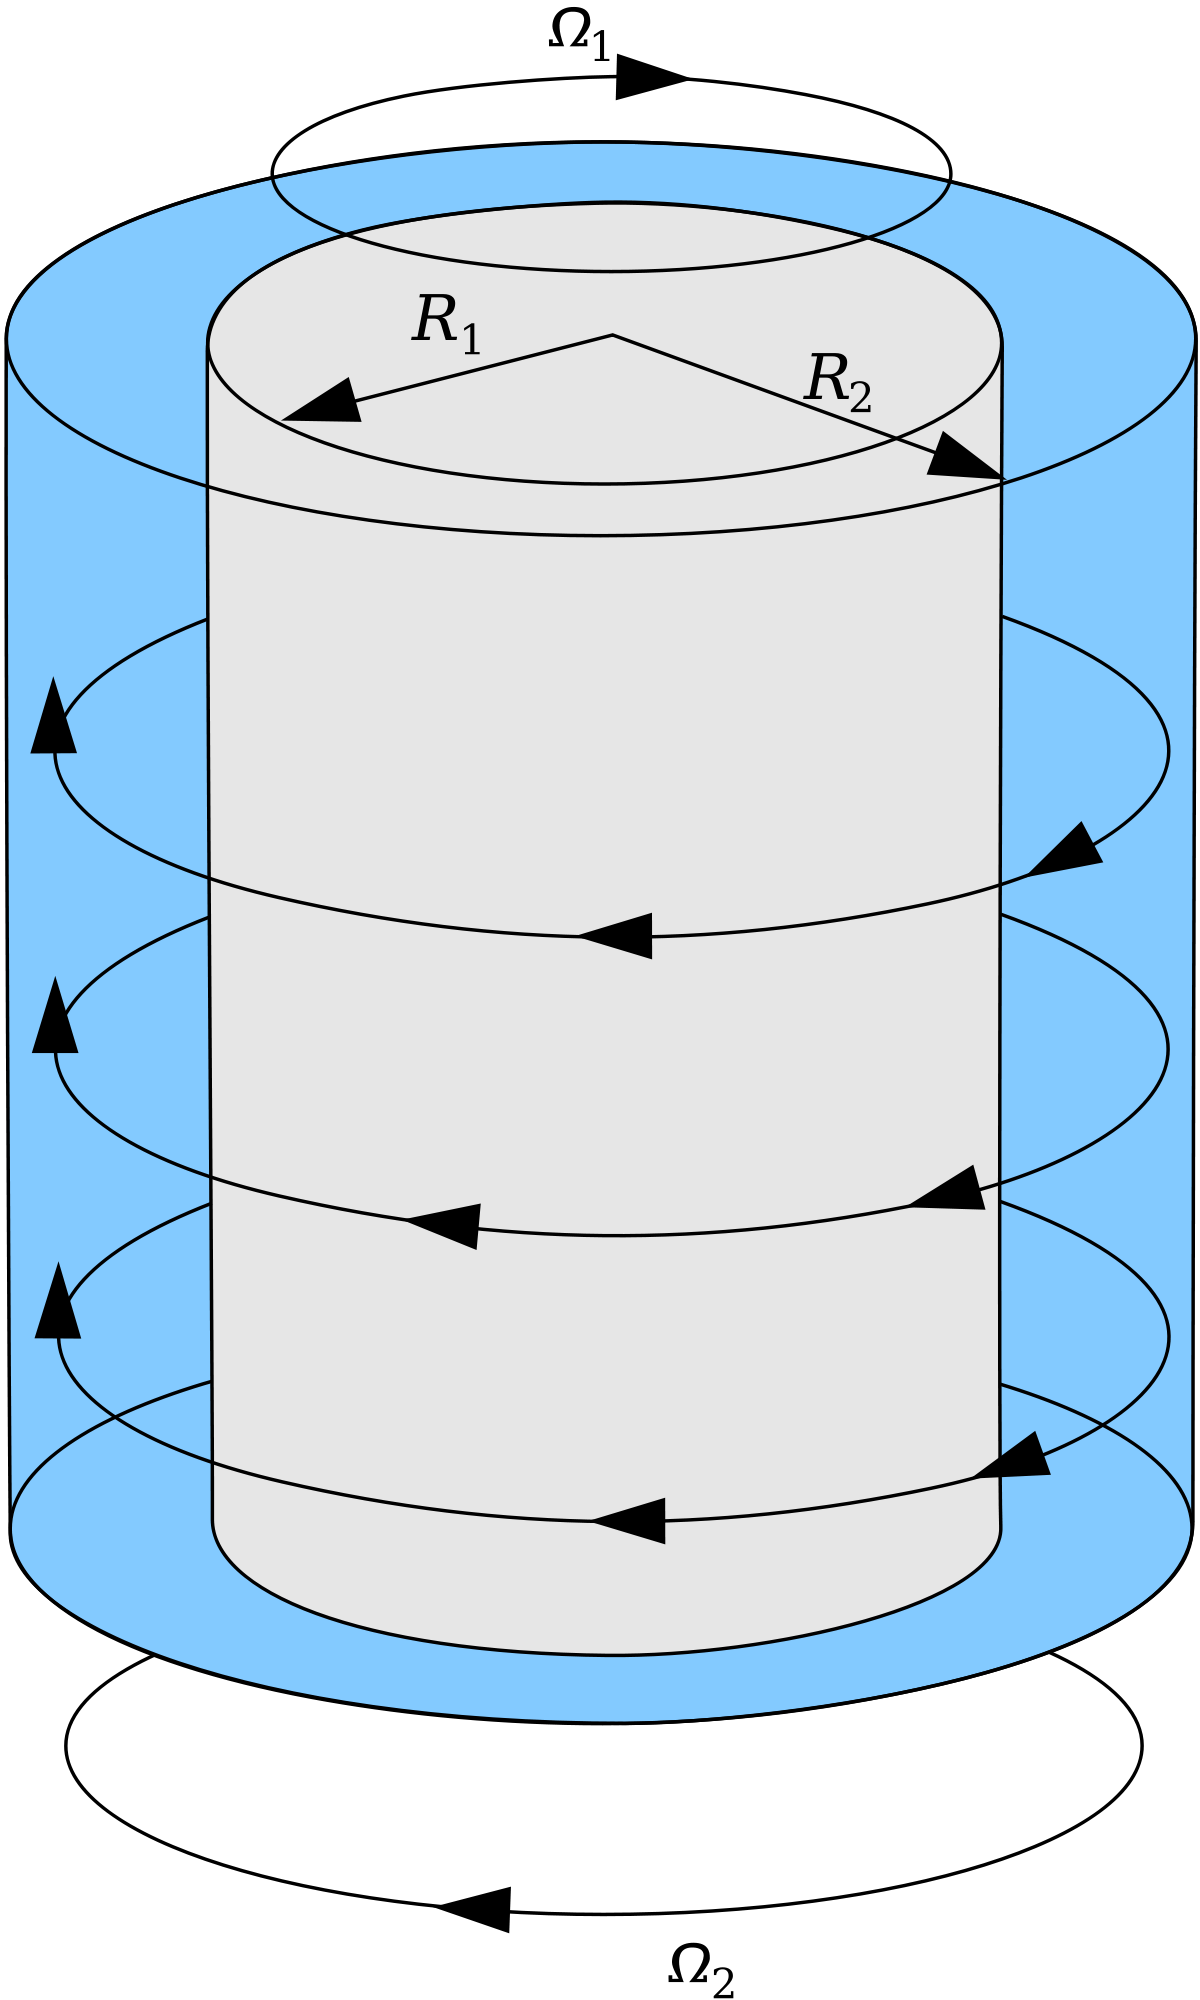
\includegraphics[scale=0.1]{1200px-CouetteTaylorSystem.svg.png}
\caption{\label{fig:def}Illustration of the definition\cite{picflow}}
\end{figure}
The described \(\Omega_1\) and \(\Omega_2\) in the picture are the angular velocities, not to mix up with the submanifold \(\Omega\). It is our goal now to compute the fluid flow inside this domain \(\Omega\).
\subsection{Physical Background}
We start with deriving the physical frame, namely the (Navier-)Stokes-Equations for incompressible fluids. For this, we need a few physical laws and mathematical theorems\cite{gibiNavier} \cite{NumFlow}[§1,§2] \cite{MoSi21}.
\subsubsection{Continuity Equation}
To derive the continuity equation, one has to use a combination of the Reynold Transport Theorem [\ref{A1}], the Gauß Theorem (or Divergence Theorem), the product rule and the fundamental lemma of calculus getting (with \(\Phi \in \mathcal{C}^{\infty}(Q,\mathbb{R}), Q:=\{(t,x)\, | \, t \in [0,T],\, x \in \Omega\}\)):
\begin{equation}
    \partial_t \Phi + \text{div}(\Phi u) = 0
\end{equation}
Where u(t,\textbf{x}) describes the velocity of the system.
\subsubsection{Conservation of Mass}
In a natural way, the mass m of a system cannot be destroyed over time, i.e. we want the following:\\
\begin{equation}
    0 = \frac{dm(t)}{dt} = \frac{d}{dt} \int_{\Omega(t)} \rho (t,\textbf{x}) \, d\lambda^n \stackrel{\ref{A1}}{=} \int_{\Omega(t)} \partial_t \rho + \text{ div}(\rho u) \, d\lambda^n
\end{equation}
We're now getting the equation of continuity for the density \(\rho\):
\begin{equation}
    \partial_t \rho + \text{div}(\rho u) = 0
\end{equation}
\subsubsection{Material Derivative}
We will describe our system in the Lagrangian way using the material derivative, sometimes also called Lagrangian derivative:
\begin{equation}
    \frac{Du}{Dt} = \partial_t u + (u \cdot \nabla)u
\end{equation}
\textbf{Note:} We can apply the material derivative to u here, because it is macroscopic (this means, that u only depends on the time t and spacial dimensions). The second term on the right side is meant to be the directional derivative of u along itself as vectorfield:
\begin{equation}
    ((u \cdot \nabla)u)_i = u_j\partial_j u_i \stackrel{(*)}{=} \text{div}((u\otimes u))_i
\end{equation}
Here (*) only holds in incompressible cases as we consider in this paper.
\subsubsection{Conservation of Momentum}
Naturally we want a second conservation to the mass, namely of the momentum I. For this we take Newton's second law (F=ma), the chain rule and the material derivative together getting for the body force b:
\begin{equation}
    b = \rho \frac{Du}{Dt}
\end{equation}
By momentum we mean the following:
\begin{equation}
    I(t) := \int_{\Omega(t)} \rho u \,\, d\lambda^n
\end{equation}
\subsubsection{Equations of Motion}
If we have a closer look at the body force we have, we see that it is a combination of fluid stresses and external forces getting:
\begin{equation}
    b = div(\sigma) + f
\end{equation}
Where f is the external force and \(\sigma\) the so called stress tensor defined by:
\begin{equation}
    \sigma := \begin{pmatrix}
\sigma_{xx} & \tau_{xy} & \tau_{xz}\\
\tau_{yx} & \sigma_{yy} & \tau_{yz}\\
\tau_{zx} & \tau_{zy} & \sigma_{zz}
\end{pmatrix}
\end{equation}
Since this definition and use of it for the Navier-Stokes-Equations seems a bit arbitrary, we should explain it more intuitively:\\
First recall that a tensor of order m is a linear map of an m-vector-tupel from an n-dimensional space into a scalar space (so a generalization of matrices). So e.g. a (Euclidean) vector is a tensor of order 1, a matrix \(A_{ij}\) of order 2. The stress tensor is also a tensor of order 2, because it has 2 directions (stress component and surface normal upon which the stress acts). The divergence of it results in a momentum source (force).
\subsubsection{Navier-Stokes Fluids}
For fluids we can partition the stress tensor into:
\begin{equation}
    \sigma = -p\mathbb{1} + T
\end{equation}
where T is the stress deviator tensor and p(t,\textbf{x}) the pressure.\\
We can define T as follows, because we have a Newtonian fluid (source was an experiment as often in physics):
\begin{equation}
    T := \mu (\nabla u + \nabla u^T)
\end{equation}
where \(\mu\) is called the viscosity of the fluid.\\
With these definitions one can calculate:
\begin{equation}
    (\text{div} \,\sigma)_i = \mu \Delta u
\end{equation}
With the whole knowledge of this chapter we can now formulate the Navier-Stokes-Equations for incompressible (Newtonian) fluids:
\begin{equation}
\begin{cases}
\rho \frac{Du(t,\textbf{x})}{Dt} + \nabla p(t,\textbf{x}) - \mu \Delta u(t,\textbf{x}) = f \\
\text{div}\, u(t,\textbf{x}) = 0
\end{cases}
\end{equation}
\textbf{Note:} The term \(-\mu \Delta u\) has a physical interpretation. It's the viscous dissipation.
\newpage
\subsection{Stokes-Equations}
For the Taylor-Couette Flow we don't need the whole complicated Navier-Stokes-Equations. Since we rotate the cylinders at low speed and have a fluid with high viscosity, we can neglect the term \((u \cdot \nabla u)\). Also we have a stationary problem, so that \(\partial_t u=0\). Under these assumptions we're now receiving the so called Stokes-Equations:\\
\pgfsetfillopacity{0.2}\colorbox{defblue}{\begin{minipage}{15cm}{\textcolor{black}{\pgfsetfillopacity{1}}{\label{def1.1}}}
\textbf{Definition 1.1 \cite{scalingRey}[§11,page 2],\cite{GaldiNavierStokes}[§4,pages 231-247]:} Let \(u:\mathbb{R}^3 \stackrel{open}{\supset} \Omega \to \mathbb{R}^3\) be the velocity of the system and \(p \in L^2_0(\Omega) := \{p \in L^2(\Omega) \, | \, \int_{\Omega} p(x)\, dx = 0\}\) the pressure. In this setting we get the so called incompressible stationary Stokes-Equations (with no external forces):
\begin{equation}
\begin{cases}
    -\mu \Delta u(t,\textbf{x}) + \nabla p(t,\textbf{x}) = 0, \text{ in } \Omega\\
    \text{div}\,u(t,\textbf{x}) = 0, \text{ in } \Omega\\
    u(t,\textbf{x}) = u_D, \text{ on } \partial \Omega
\end{cases}
\end{equation}
\end{minipage}}\\

\textbf{Note:} We formulated the equations with Dirichlet boundary conditions because this is a proper setting for the Taylor-Couette Flow. \\Lastly we chose \(L^2_0(\Omega)\) as space for the pressure to fix the non-uniqueness of p (it's just an uniqueness up to a constant; one can show the fix with some Functional Analysis (saddle point theory) but this would need too much introduction to be reasonable here.).
\newpage
\section{Analytical solution for symmetry case}
We will now present an analytical solution for comparison later. It is natural to use cylindrical coordinates:\\
\pgfsetfillopacity{0.2}\colorbox{defblue}{\begin{minipage}{15cm}{\textcolor{black}{\pgfsetfillopacity{1}}{\label{def1.2}}}
\textbf{Definition and lemma 1.2:} Consider a map
\begin{equation}
    \Phi : \mathbb{R}^+ \,\times ]0,2\pi] \times \mathbb{R} \to \mathbb{R}^3,\,
    \Phi (r,\phi,z):=(r\cdot cos(\phi),r\cdot sin(\phi),z)^T
\end{equation}
We call this map cylindrical coordinates. If we consider then:
\begin{equation}
    (x,y,z) \in \Omega \mapsto (r,\phi,z)
\end{equation}
We can say then, that (1.3) using (1.2) is a \(\mathcal{C}^{\infty}\)-diffeomorphism. 
\end{minipage}}\\

\textsc{Proof:} This is a standard result from Calculus 3, see for example: \cite{ElstrodtAna3}[§4,page 225]. \QEDB\\
\textbf{Note:} It's equivalent to use \([0,2\pi]\) for \(\phi\), because a point in \(\mathbb{R}^3\) has Lebesgue-measure 0. This is important for the validation of the injectivity!\\

We will need a second lemma for solving the equation:\\
\pgfsetfillopacity{0.2}\colorbox{lemyellow}{\begin{minipage}{15cm}{\textcolor{black}{\pgfsetfillopacity{1}}{\label{lem1.3}}}
\textbf{Lemma 1.3:} For cylindrical coordinates u we get the following properties:
\begin{enumerate}
%\begin{equation}
    \item $\nabla u = \partial_rue_r + \frac{1}{r}\partial_{\phi}ue_{\phi} + \partial_zue_z$
    \item $\text{div }u = \frac{1}{r}\partial_r(ru_r) + \frac{1}{r}\partial_{\phi}u_{\phi} + \partial_zu_z$
    \item $\Delta u = \frac{1}{r}\partial_r(r\partial_ru) + \frac{1}{r^2}\partial_{\phi \phi}u + \partial_{zz}u$
    \item $(u \cdot \nabla)u = \frac{1}{2}\nabla ||u||^2 - u \times curl\, u$
%\end{equation}
\end{enumerate}
\end{minipage}}\\

\textsc{Proof:} 1.-3. are straightforward calculations with the useful fact from [\ref{def1.2}][Lemma 1.2].\\
For 4. use the following property for vectorfields a and b in \(\mathbb{R}^3\):
\begin{equation}
    \nabla(a \cdot b) = a \times (\nabla \times b) + b \times (\nabla \times a) + (a \cdot \nabla)b + (b \cdot \nabla)a
\end{equation}
This completes the proof. \QEDB\\
\newpage
With this knowledge in mind we can now present the analytical solution for a symmetry case (we reduce the problem to a two-dimensional one within symmetry arguments, considering infinite long cylinders):\\
\pgfsetfillopacity{0.2}\colorbox{theored}{\begin{minipage}{15cm}{\textcolor{black}{\pgfsetfillopacity{1}}}
\textbf{Theorem 1.4:} Assume that we just have a movement in direction of the angulars, i.e. it holds:
\begin{equation}
\begin{array}{l}
    u(x,y,z) = u_{\phi}(r_i) := r_i \cdot \Omega_i,\, i=1,2\\
    u_r(r_i) = u_z(r_i) = 0,\, i=1,2
\end{array}
\end{equation}
Assuming \(p(x,y,z)=p(r)\) for the pressure, the solution has the form:
\begin{equation}
    u_{\phi} = r \cdot \frac{r_2^2\cdot \Omega_2 - r_1^2\cdot \Omega_1}{r_2^2 - r_1^2} + (\Omega_1 - \Omega_2)\cdot \frac{1}{r} \cdot \frac{r_1^2 \cdot r_2^2}{r_2^2 - r_1^2}
\end{equation}
\end{minipage}}\\

\textsc{Proof:} With the symmetry assumptions and [\ref{lem1.3}][Lemma 1.3] we directly get:
\begin{enumerate}
    \item $\text{div }u = 0$
    \item $\text{curl }u = \frac{1}{r}\partial_r(ru_{\phi}(r))e_z$
\end{enumerate}
Using the 2 properties in [\ref{def1.1}][Definition 1.1], we finally get our differential equation, we can easily solve (for more details and why we need (2.), see: \cite{solproof}):
\begin{equation}
    \partial_r(\frac{1}{r}\partial_r(ru_{\phi})) = 0
\end{equation}
Since this differential equation only depends on r, we have a homogenous ODE, which we can solve by just integrating twice. The solution is our assertion. \QEDB\\

Because we want to simulate this setting (infinite long cylinders, so ignoring the dependence on z) in the following, we should write it down explicitly, this time \textbf{with} external forces:\\
\begin{equation}
\begin{cases}
-\mu (\frac{1}{r}\partial_r(r\partial_r u_r) + \frac{1}{r^2}\partial_{\phi \phi} u_r) + \partial_r p = f_r, \text{ in }\Omega\\
-\mu (\frac{1}{r}\partial_r(r\partial_r u_{\phi}) + \frac{1}{r^2}\partial_{\phi \phi} u_{\phi}) + \frac{1}{r}\partial_{\phi} p = f_{\phi}, \text{ in }\Omega\\
\text{div }u = 0,\text{ in }\Omega\\
u_r = u_z = 0, \text{ on }\partial \Omega\\
u_{\phi} = u_D, \text{ on }\partial \Omega
\end{cases}
\end{equation}
\chapter{DISCRETIZATION}
The inspiration for the whole chapter 2 was taken out of \cite{numFlowSaddle}.
\section{Variational Form}
Before we can model our problem, we need the weak form of the Stokes-Equations first. Here we will no longer assume, that there are no external forces, because this leads to a non-realistic simulation.\\

\pgfsetfillopacity{0.2}\colorbox{defblue}{\begin{minipage}{15cm}{\textcolor{black}{\pgfsetfillopacity{1}}{\label{def2.1}}}
\textbf{Definition 2.1:} Using a test function \(\varphi \in \mathring{W}^{1,2}(\Omega)^n\) integrating with Green's Theorem, we receive the mixed weak formulation of the Stokes-Equations:
\begin{equation}
    \begin{array}{l}
    a(u,\varphi) + b(p,\varphi) = <f,\varphi>\,\, \forall \varphi \in \mathring{W}^{1,2}(\Omega)^n, \, f \in (\mathring{W}^{1,2}(\Omega)^n)'\\
    b(q,u) = 0\,\, \forall q \in L^2_0(\Omega)
    \end{array}
\end{equation}
Here a and b are defined as:
\begin{equation}
    \begin{array}{l}
    a(u,\varphi) := \mu \int_{\Omega} \nabla u \cdot \nabla \varphi \, d\lambda^n\\
    b(q,\varphi) := -\int_{\Omega} q \cdot \text{div}(\varphi)\, d\lambda^n
    \end{array}
\end{equation}
\end{minipage}}\\

\textbf{Note:} Problem (2.1) has an unique solution. Since the proof for that is really technical, we abstain from a proof. See \cite{NecasSol} for more details. Keep in mind that we're looking at Lipschitz boundaries (\(\partial \Omega \in \mathcal{C}^{0,1}\)), for which we have such a proof in general.
\newpage
\section{Standard Approach}
Before we start with first approaches, we should recall what we need to get a stable numerical solution. We will abbreviate for better reading \(X:=\mathring{W}^{1,2}(\Omega)^n, \, Y:=L^2_0(\Omega)\) getting:\\
\pgfsetfillopacity{0.2}\colorbox{defblue}{\begin{minipage}{15cm}{\textcolor{black}{\pgfsetfillopacity{1}}{\label{def2.2}}}
\textbf{Definition and lemma 2.2 \cite{NumFlow}:} Let \(X_h \subset X, \, Y_h \subset Y\). \\We're searching for a solution \((u_h,p_h) \in X_h \times Y_h\), s.t. it holds:
\begin{equation}
\begin{cases}
    a(u_h,\varphi_h) + b(p_h,\varphi_h) = <f,\varphi_h> \,\, \forall \varphi_h \in X_h\\
    b(q_h,u_h) = 0 \,\, \forall q_h \in Y_h
\end{cases}
\end{equation}
This solution is unique iff it holds:
\begin{enumerate}
    \item $\sup\limits_{0 \neq x_0 \in V_{0,h}} \frac{|a(\varphi_0,x_0)|}{||x_0||_X} \geq \alpha_h ||\varphi_0||_X\,\, \forall \varphi_0 \in V_{0,h}$
    \item $\sup\limits_{0 \neq \varphi_h \in X_h} \frac{|b(q_h,\varphi_h)|}{||\varphi_h||_X} \geq \beta_h ||q_h||_Y\,\, \forall q_h \in Y_h$
\end{enumerate}
Or equivalently:
\begin{enumerate}
    \item $\inf\limits_{0\neq \varphi_0 \in V_{0,h}}\,\,\sup\limits_{0 \neq x_0 \in V_{0,h}} \frac{|a(\varphi_0,x_0)|}{||x_0||_X\,||\varphi_0||_X} \geq \alpha_h$
    \item $\inf\limits_{0\neq q_h \in Y_h}\,\,\sup\limits_{0 \neq \varphi_h \in X_h} \frac{|b(q_h,\varphi_h)|}{||\varphi_h||_X \, ||q_h||_Y} \geq \beta_h$
\end{enumerate}
With \(V_{0,h} := \{v_h \in X_h \, | \, b(q_h,\varphi_h) = 0 \,\,\forall q_h \in Y_h\}, \, \alpha_h, \beta_h > 0.\)
\end{minipage}}\\

\textbf{Note:} The second condition (for b) is equivalent to the surjectivity of B, the operator to b, defined by:
\begin{equation}
    <Bq_h,\varphi_h> := b(q_h,\varphi_h)
\end{equation}
The idea of the proof of it is of course that we get the needed invertibility of the system with these conditions.\\

Our first approach is now the naive one: we're using \(\mathcal{P}_1 \times \mathcal{P}_0\) as the space for the solution in \(X_h \times Y_h\). However, we will get a big problem here\cite{brezzi}:\\
Consider NT triangles, N interior and M boundary nodes. We have then NT-1 degrees of freedom (dof) for the pressure (since one is determined by demanding \(\int_{\Omega} p(x) dx = 0\)) and 2N dof for the velocity (since we are using finite elements that should vanish on the boundary). The following image illustrates the mesh and dof:
\begin{figure}[H]
\centering
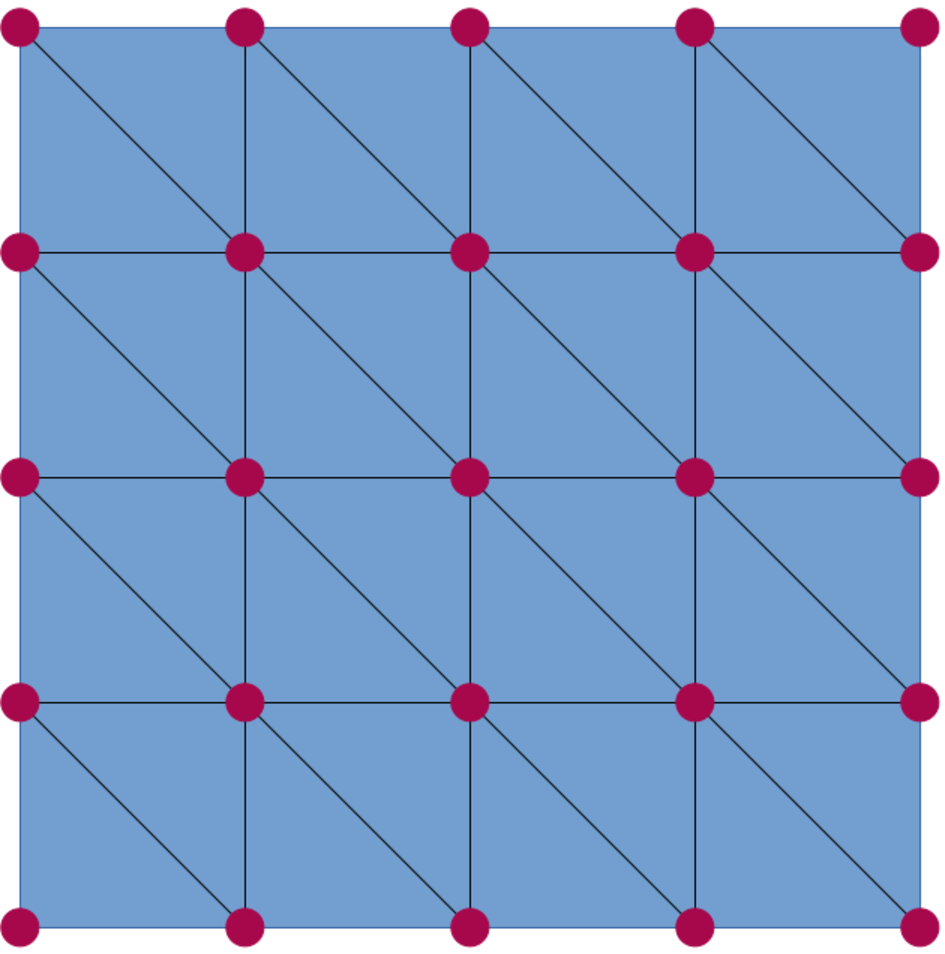
\includegraphics[scale=0.5]{TriangleMeshStokes.pdf}
\caption{\label{fig:mesh}Illustration of the mesh}
\end{figure}
Recall now Euler's equation for finite planar graphs:
\begin{equation}
    NT = 2N + M - 2
\end{equation}
By definition of our finite elements it holds \(M>3\), so that we get:
\begin{equation}
    NT - 1 > 2N
\end{equation}
We need B to be surjective, so rank(B) = NT. But this is impossible because of (2.6)!\\
This shows that the naive Finite Elements Space for our problem is too "small", so we will need another approach.\\
\textbf{Note:} The approach \(\mathcal{P}_1 \times \mathcal{P}_1\) fails in an analog way: one can construct triangles with nodes -1,1,0 getting 0 calculating (in \(\mathcal{P}_1\) exactly!) the integral in b with the midpoint rule.
\newpage
\section{Taylor-Hood Approach}
What we will use as an second approach, is the so called "Taylor-Hood-Approach". This means, we're using \(\mathcal{P}_k \times \mathcal{P}_{k-1}\) as space for the solution, \(k \geq 2\). The resulting numerical procedure is indeed stable then (see the following) and one can show with some Calculus that it also has an optimal convergence rate, see \ref{A2}. We will use \(k=2\):\\
\pgfsetfillopacity{0.2}\colorbox{theored}{\begin{minipage}{15cm}{\textcolor{black}{\pgfsetfillopacity{1}}{\label{theo2.3}}}
\textbf{Theorem 2.3:} Consider problem (2.3) in [\ref{def2.2}][Definition 2.2]. If we use:
\begin{equation}
    X_h := \mathcal{P}_2,\, Y_h := \mathcal{P}_1
\end{equation}
(on triangles) then [\ref{def2.2}][Lemma 2.2] holds.
\end{minipage}}\\

\textsc{Proof:} See \cite{taylorhood}. Note that we reduced our problem to a two dimensional one, so the proof here is valid for our problem. \QEDB

More concrete we define our spaces for a family of triangulations \((\mathcal{T}_h)_h\)\cite{taylorhood}:
\begin{equation}
\begin{array}{l}
X_h := \{u \in (\mathcal{C}^0(\Omega))^2 \,|\, u_D = 0, u_{\einschraenkung T} \in (\mathcal{P}_2(T))^2,\, T \in (\mathcal{T}_h)_h\} \\
Y_h := \{p \in \mathcal{C}^0_0(\Omega)\,|\, p_{\einschraenkung T} \in  \mathcal{P}_1(T)\}
\end{array}
\end{equation}
\textbf{Note:} Here \(\mathcal{C}^0_0(\Omega)\) has the same additional property as \(L^2_0(\Omega)\).
\section{Galerkin Approximation}
Now we will use Galerkin approximation getting a system we can implement later. Doing some calculations, this is the weak system we want to solve for all \( u,v \in X_h, \\p,q \in Y_h,\, \Omega := \mathbb{R}^+ \times [0,2\pi]\):\\
\begin{gather}
\begin{cases}
    \mu \iint_{\Omega} r \partial_r v_r \partial_r u_r \, dr\,d\phi + \mu \iint_{\Omega} \frac{1}{r} \partial_{\phi} v_r \partial_{\phi} u_r \, dr\,d\phi - \iint_{\Omega} rp \partial_r v_r \, dr\,d\phi =\\
    \quad \iint_{\Omega} r(f_r v_r) \, dr\,d\phi\\
    \mu \iint_{\Omega} r \partial_r v_{\phi} \partial_r u_{\phi} \, dr\,d\phi + \mu \iint_{\Omega} \frac{1}{r} \partial_{\phi} v_{\phi} \partial_{\phi} u_{\phi} \, dr\,d\phi - \iint_{\Omega} p \partial_{\phi} v_{\phi} \, dr\,d\phi =\\
    \quad \iint_{\Omega} r(f_{\phi} v_{\phi}) \, dr\,d\phi\\
    \iint_{\Omega} rq\partial_r u_r \, dr\,d\phi + \iint_{\Omega} rq\partial_{\phi} u_{\phi} \, dr\,d\phi = 0
\end{cases}
\end{gather}
Remember here that we had to insert an r as the Jacobian of the transformation.\\

Now we need a basis for \(X_h\), called N and a basis for \(Y_h\), called M. Here we use the Taylor-Hood-Approach. Define N and M elementwise, so choose shape functions for the master elements (which are quadratic elements):
\begin{equation}
N^e (\xi,\eta) :=
\begin{bmatrix}
(1-\xi)(1-2\xi)(1-\eta)(1-2\eta)\\
(2\xi-1)\xi(1-\eta)(1-2\eta)\\
(2\xi-1)\xi(2\eta-1)\eta\\
(1-\xi)(1-2\xi)(2\eta-1)\eta\\
4(1-\xi)\xi(1-\eta)(1-2\eta)\\
(2\xi-1)\xi4(1-\eta)\eta\\
4(1-\xi)\xi(2\eta-1)\eta\\
(1-\xi)(1-2\xi)4(1-\eta)\eta\\
4(1-\xi)\xi4(1-\eta)\eta
\end{bmatrix}^T
,\, M^e (\xi,\eta) :=
\begin{bmatrix}
(1-\xi)(1-\eta)\\
\xi(1-\eta)\\
\xi \eta\\
(1-\xi)\eta
\end{bmatrix}^T
\end{equation}
Basically, this is what we are considering now:
\begin{figure}[H]
\centering
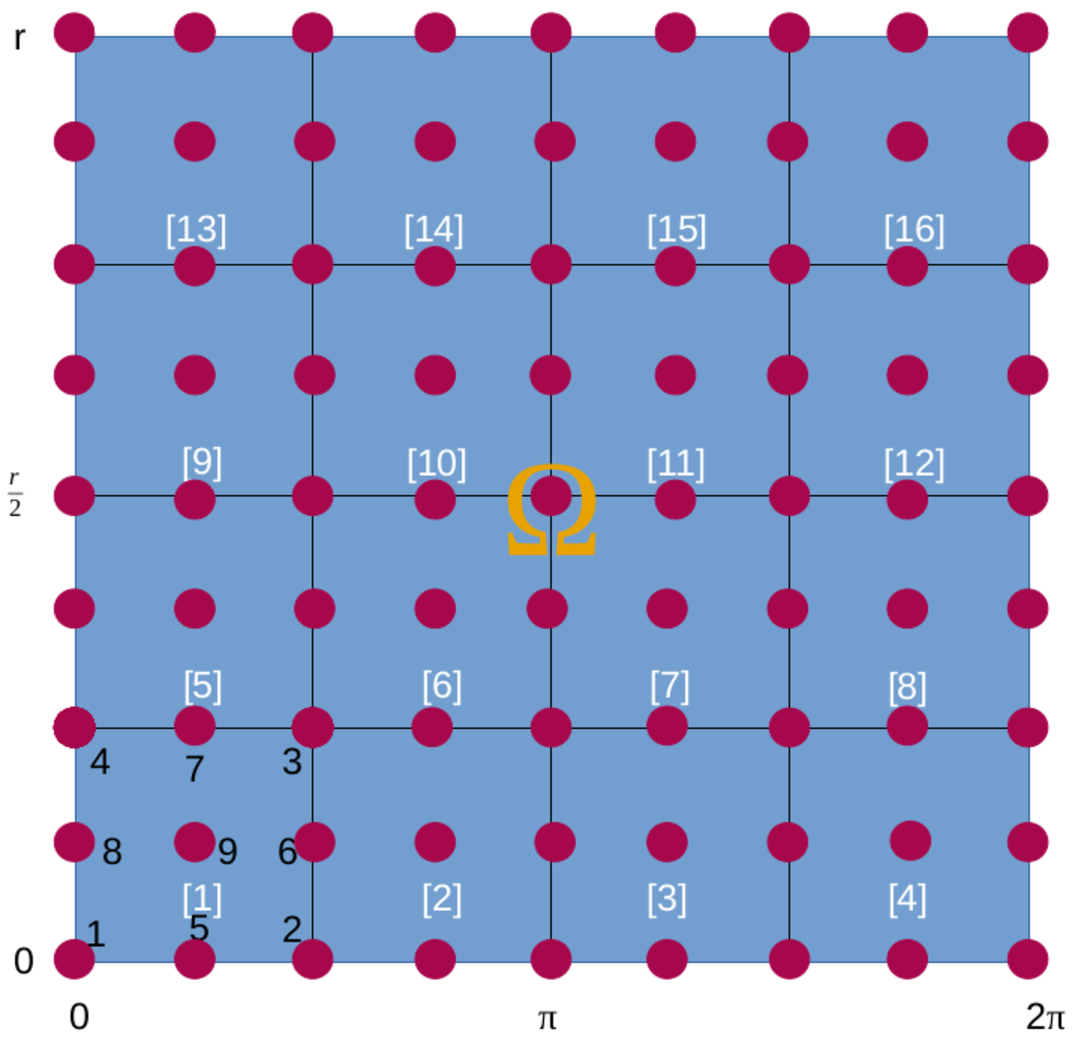
\includegraphics[scale=0.5]{TrMeshStokes3.pdf}
\caption{\label{fig:meshCou}Illustration of the mesh for \(\phi = 2\pi\)}
\end{figure}
With these bases we can write:
\begin{equation}
\begin{array}{l}
    u_{N,r} = u_{h,r}= Nu_r\\
    u_{N,\phi} = Nu_{\phi}\\
    v_{N,r} = v^T_r N^T\\
    v_{N,\phi} = v^T_{\phi} N^T\\
    p_M = Mp\\
    q_M = q^T M^T
\end{array}
\end{equation}
So (2.9) is now:
\begin{gather}
    \begin{cases}
        \mu \iint_{\Omega}rv^T_r \frac{\partial N^T}{\partial r}\frac{\partial N}{\partial r} u_r\, dr\,d\phi + \mu \iint_{\Omega} \frac{1}{r}v^T_r \frac{\partial N^T}{\partial \phi} \frac{\partial N}{\partial \phi} u_r\, dr\,d\phi - \iint_{\Omega} rv^T_r \frac{\partial N^T}{\partial r}Mp\, dr\,d\phi =\\
        \quad \iint_{\Omega} rv^T_rN^Tf_r \, dr\,d\phi\\
        \mu \iint_{\Omega}rv^T_{\phi} \frac{\partial N^T}{\partial r}\frac{\partial N}{\partial r} u_{\phi}\, dr\,d\phi + \mu \iint_{\Omega} \frac{1}{r}v^T_{\phi} \frac{\partial N^T}{\partial \phi} \frac{\partial N}{\partial \phi} u_{\phi}\, dr\,d\phi - \iint_{\Omega} v^T_{\phi} \frac{\partial N^T}{\partial \phi}Mp\, dr\,d\phi =\\
        \quad \iint_{\Omega} rv^T_{\phi}N^Tf_{\phi} \, dr\,d\phi\\
        \iint_{\Omega} rq^T M^T\frac{\partial N}{\partial r} u_r \,dr\,d\phi + \iint_{\Omega} rq^T M^T \frac{\partial N}{\partial \phi} u_{\phi} \,dr\,d\phi = 0
    \end{cases}
\end{gather}
Or in matrix form:\\
\begin{equation}
\begin{bmatrix}
v^T_r & v^T_{\phi} & q^T
\end{bmatrix}
\begin{bmatrix}
A_{11} & 0 & A_{13}\\
0 & A_{11} & A_{23}\\
A^T_{13} & A^T_{23} & 0
\end{bmatrix}
\begin{bmatrix}
u_r\\
u_{\phi}\\
p
\end{bmatrix}
=
\begin{bmatrix}
v^T_r & v^T_{\phi} & 0
\end{bmatrix}
\begin{bmatrix}
F_{11} & 0 & 0\\
0 & F_{11} & 0\\
0 & 0 & F_{11}
\end{bmatrix}
\begin{bmatrix}
f_r\\
f_{\phi}\\
0
\end{bmatrix}
\end{equation}\\
With entries:
\begin{equation}
\begin{array}{l}
    A_{11} := \mu \iint_{\Omega}r \frac{\partial N^T}{\partial r}\frac{\partial N}{\partial r} \, dr\,d\phi + \mu \iint_{\Omega} \frac{1}{r} \frac{\partial N^T}{\partial \phi} \frac{\partial N}{\partial \phi} \, dr\,d\phi\\
    A_{13} := - \iint_{\Omega} r \frac{\partial N^T}{\partial r}M\, dr\,d\phi\\
    A_{23} := - \iint_{\Omega} \frac{\partial N^T}{\partial \phi}M\, dr\,d\phi\\
    F_{11} := \iint_{\Omega} rN^T \, dr\,d\phi
\end{array}
\end{equation}
\chapter{SIMULATION USING FINITE ELEMENTS}
Now we can start with the simulation part. We will do that by writing a matlab program (available as an extra file of course, code will not be attached here). In the following we will just show the plots the program generates and give some explanations to the procedure and the ideas in the code.\\

The algorithm is a straightforward implementation of chapter 2. In step 3 we compute the element matrices for A and F. Here we first transform the resulting integrals of the entries of A and F to the reference element and transform it back in step 4 when building A and F out of their element matrices.\\
Keep in mind that in step 5 of the algorithm, where we insert the boundary conditions, we have only conditions for \(u_{\phi}\). The conditions appear at the first and last row of nodes, so our boundary conditions are the angular velocities \(\Omega_1, \Omega_2\), see \ref{fig:def}.
\newpage
Now we show plots of the simulation. Here we used the algorithm for the following setting:
\begin{equation}
    \begin{array}{l}
         \mu = 48.8 \,mPas\\
         r_1 = 5 \, m, \, r_2 = 6 \, m\\
         \Omega_1 = 10 \, \frac{m}{s}, \, \Omega_2 = 20 \, \frac{m}{s}\\
         \#\{R-MeshNodes\} = 25, \, \#\{\phi-MeshNodes\} = 50\\
         \phi = 2\pi\\
         f(r,\phi) = (r^2+\phi ^2,r)
    \end{array}
\end{equation}\\
The value of \(\mu\) conforms sunflower oil, see: \cite{visc}.\\
The plots look like that then:\\

\begin{figure}[H]
\centering
\begin{minipage}{.5\textwidth}
  \centering
  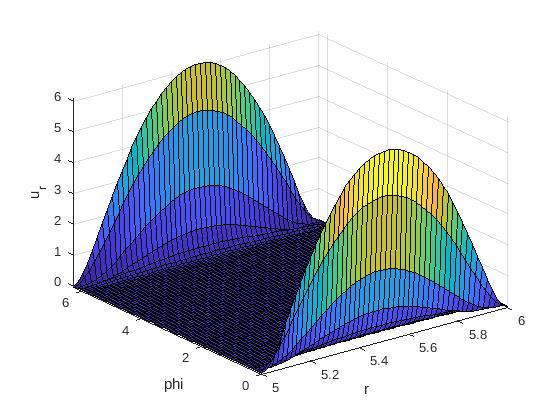
\includegraphics[width=1.2\linewidth]{UrFcircle.jpg} 
  \caption{Graph of \(u_r\) in the setting}
  \label{fig:plot1}
\end{minipage}%
\begin{minipage}{.5\textwidth}
  \centering
  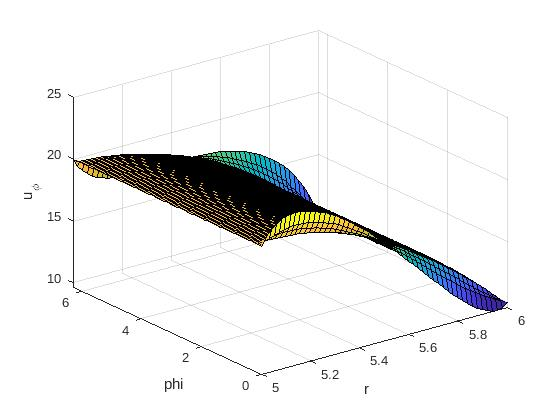
\includegraphics[width=1.2\linewidth]{UphiFcircle.jpg}
  \caption{Graph of \(u_{\phi}\) in the setting}
  \label{fig:plot2}
\end{minipage}
\end{figure}
\begin{figure}[H]
\centering
\begin{minipage}{.5\textwidth}
  \centering
  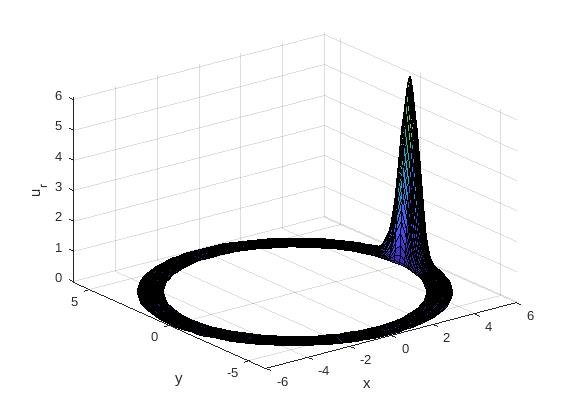
\includegraphics[width=1.2\linewidth]{MeshUrFcircle.jpg} 
  \caption{Mesh of \(u_r\) in the setting}
  \label{fig:plot3}
\end{minipage}%
\begin{minipage}{.5\textwidth}
  \centering
  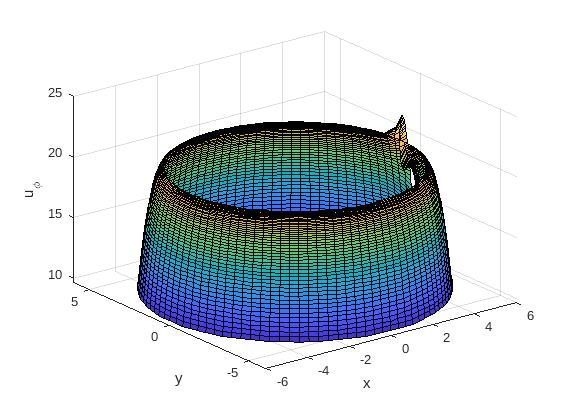
\includegraphics[width=1.2\linewidth]{MeshUphiFcircle.jpg}
  \caption{Mesh of \(u_{\phi}\) in the setting}
  \label{fig:plot4}
\end{minipage}
\end{figure}
\addcontentsline{toc}{chapter}{Appendices}
\chapter*{\centering \large Appendix\markboth{Appendix}{Appendix}}
\pgfsetfillopacity{0.2}\colorbox{theored}{\begin{minipage}{15cm}{\textcolor{black}{\pgfsetfillopacity{1}}{\label{A1}}}
\textbf{Theorem A.1:} (Reynold Transport Theorem) \\
Let \(\Phi \in \mathcal{C}^{\infty}(Q,\mathbb{R}), Q:=\{(t,x)\, | \, t \in [0,T],\, x \in \Omega\}\), n be the outer unit normal vector. Then it holds:
\begin{equation}
    \frac{d}{dt}\int_{\Omega(t)} \Phi\, \,d\lambda^3 = \int_{\partial \Omega(t)} \Phi u \cdot n \, \,d\mathcal{H}^2 + \int_{\Omega(t)} \frac{\partial \Phi}{\partial t} \, \,d\lambda^3
\end{equation}
\end{minipage}}\\

\textbf{Notes:} \begin{enumerate}
    \item This is not trivial, since the domain depends on t! 
    \item In general the statement has to involve \(u = u_s\), so the velocity on the surface. But in fluid dynamics we look at accumulations of the fluid, where mass is not changing (see chapter 1), so it holds: \(u \cdot n = u_s \cdot n\).
    \item There is of course a dependence between \(\Phi\) and \(u\). It's called the material derivative (used also in the proof of the theorem):\begin{equation}
        \frac{D \Phi(t,\textbf{x})}{Dt} = \frac{\partial  \Phi(t,\textbf{x})}{\partial t} + \nabla \Phi(t,\textbf{x}) \cdot u(t,\textbf{x})
    \end{equation}
\end{enumerate}
\pgfsetfillopacity{0.2}\colorbox{theored}{\begin{minipage}{15cm}{\textcolor{black}{\pgfsetfillopacity{1}}{\label{A2}}}
\textbf{Theorem A.2 \cite{calcStokes}[Theorem 3.1]:} (Convergence rate of Taylor-Hood-Elements in Stokes-Equations)\\
Let (u,p) be a solution of \ref{def1.1}, \((u_h,p_h)\) of \ref{def2.1} and \((e_u,e_p)\) the consequential errors of the weak problem (both problems with external forces). \\Then there exist constants \(C_1,C_2,C_3,C_{\mathcal{T}}\) such that:
\begin{equation}
\begin{array}{l}
    C_2||(e_u,e_p)||_{X \times Y} + \frac{1}{2\sqrt{n}}||\text{div }u_h||_{X} \le ||(u-u_h,p-p_h)||_{X \times Y}\\ \le C_3 ||(e_u,e_p)||_{X \times Y} + \frac{1}{C_1}||\text{div }u_h||_{X} + \frac{C_{\mathcal{T}}}{C_1}\sqrt{\sum_{T \in \mathcal{T}}h^2_T \, \inf_{K \in (\mathbb{P}_k(T))^3} ||f - K||^2_{0,T}}
    \end{array}
\end{equation}
\end{minipage}}\\
\addcontentsline{toc}{chapter}{References}
\printbibliography
%\bibliographystyle{plain}
\end{document}

